\documentclass[addpoints]{exam}
\usepackage{amsmath, amsfonts, amssymb, amsthm}
\usepackage{forest}
\usepackage{geometry}
\usepackage{hyperref}
\usepackage{titling}
\usepackage{tikz}

% Header and footer.
\pagestyle{headandfoot}
\runningheadrule
\runningfootrule
\runningheader{CS 212, Fall 2023}{HW 2: Pumping Lemma, Context Free Languages}{Fall 2023}
\runningfooter{}{Page \thepage\ of \numpages}{}
\firstpageheader{}{}{}

\boxedpoints
\printanswers

\title{Homework 2: Pumping Lemma, Context Free Languages}
\author{CS 212 Nature of Computation\\Habib University\\Homework 02 22}
\date{Fall 2023}

\begin{document}
\maketitle

\begin{questions}

  \question Consider the grammar containing the following productions.
  \begin{align*}
    S \to & \; XaY                      \\
    X \to & \; aX \mid \epsilon         \\
    Y \to & \; aY \mid bY \mid \epsilon
  \end{align*}

  \begin{parts}
    \part[5] Give a formal definition of the language generated by this grammar.
    \part[5] Draw the parse tree under this grammar for the string: aaaba.\footnote{ See \href{https://tex.stackexchange.com/a/214657/44301}{this post} on using the \texttt{forest} package to draw a parse tree.}
    \part[5] Argue whether this grammar is ambiguous.
  \end{parts}

  \question[5] Given an alphabet, $\Sigma$, consider the operation, $f:\Sigma^*\to\Sigma^*$, defined as follows.
  \[
    f(w) = w_n\circ w_{n-1}\circ w_{n-2}\circ\ldots w_{1}, \text{ where } w = w_1\circ w_2\circ w_3\circ\ldots\circ w_n.
  \]
  $f$ is extended to apply to a given language, $L$, as follows.
  \[
    f(L) = \{ f(w) \mid w\in L \}.
  \]
  Prove or disprove the claim that the class of context-free languages is closed under $f$.

  \question[5] Prove or disprove the claim that the language, $L=\{ x\#y \mid x,y\in\{0,1\}^*\}$, is context-free.

  \question We are given the language, $L = \{0^i1^j2^k \mid i,j,k \geq 0, k \neq 1 \text{ or } i = j\}$.
  \begin{parts}
    \part[5] Without using the pumping lemma, argue that $L$ is not regular.
    \part[5] Show that the pumping lemma for regular languages applies to $L$.
    \part[5] What conclusion can you draw about the pumping lemma from the above observations?
  \end{parts}

  \pagebreak
  \begin{solution}

    \textbf{Problem 1:}
    \begin{parts}
      \part For the language $L$, our components for its grammar becomes: \vspace*{-2mm}
      \begin{itemize}
        \item $N$ is a non empty set of non terminal symbols; $ N = \{ S, X, Y \}$
        \item $ \sum $ is a finite set of terminal symbols; $ \sum = \{ \varepsilon, a \} $
        \item $P$ is the set of grammar rules; $ P = \{ S \rightarrow XaY, X \rightarrow aX \mid \varepsilon, Y \rightarrow aY \mid bY \mid \varepsilon \} $
        \item $S \in N$ is the start symbol; $ S = S $
      \end{itemize}

      Formally the grammar for this language is, \vspace*{-2mm} $$ G = \{ \{ S, X, Y \},  \{ \varepsilon, a \}, \{ S \rightarrow XaY, X \rightarrow aX \mid \varepsilon, Y \rightarrow aY \mid bY \mid \varepsilon \}, S  \} $$

      And the language can be defined as $$ L(G) = \{ a^* (ba)^* \mid a, b \in \sum \} $$

      % The language consists of all strings over the alphabet $\{a,b\}$ that contain at least one $a$ followed by 0 or more number of $a$'s and $b$'s in any order. \\ Then $ L(G) = \{a^*(ba)^* \mid a, b \in \{a, b\} \} $
      \part The parse tree for the string $aaaba$ is as follows:
      \begin{center}
        \begin{forest}
          [S
              [X
                  [[[a]]]
                  [X
                      [[a]][X[$\varepsilon$]]
                  ]
              ]
              [[[[a]]]]
              [Y
                  [[[b]]]
                  [Y
                      [[a]][Y[$\varepsilon$]]
                  ]
              ]
          ]
        \end{forest}
      \end{center}
      \part This grammar is ambiguous because the string $aaaba$ can be parsed in different ways. One is as shown in the previous part and the other is as follows:
      \begin{center}
        \begin{forest}
          [S
              [X
                  [[[[a]]]][X[[[$\varepsilon$]]]]
              ]
              [[[[[a]]]]]
              [Y
                  [[[[a]]]]
                  [Y
                      [[[b]]]
                      [Y
                          [[a]][Y[$\varepsilon$]]
                      ]
                  ]
              ]
          ]
        \end{forest}
      \end{center}
      Therefore, the grammar is ambiguous since we have found two different parse trees for the same string.
    \end{parts}

    \newpage
    \textbf{Problem 2:}
    We are given the operation, $f:\Sigma^*\to\Sigma^*$, defined as follows:
    \[ f(w) = w_n\circ w_{n-1}\circ w_{n-2}\circ\ldots w_{1}, \text{ where } w = w_1\circ w_2\circ w_3\circ\ldots\circ w_n. \]
    Extending $f$ to a language $L$, we have: $ f(L) = \{ f(w) \mid w \in L \} $

    Essentially, $f$ reverses the order of the characters in a string. Extending $f$ to $L$ means that we apply $f$ to every string in $L$, then $f(L)$ consists of all the strings that we get by reversing each string in $L$.

    Given that $L$ is a context-free language over an alphabet $\sum$ and its context-free grammar $G$, we can assume, without loss of generality that $L$ is in Chomsky Normal Form (CNF) - if not, then we can convert it to CNF. Then all production rules are of the form $ A \rightarrow BC $, or $ A \rightarrow a $, where $ A, B, $ and $C$ are non-terminal symbols and $a$ is a terminal symbol.

    Then we construct a new grammar $G'$ that generates the language $f(L)$ which consists of the reverse of every string in $L$. The non-terminal symbols of $G'$ are the same as those of $G$, and the start symbol of $G'$ is the same as that of $G$. The production rules of $G'$ are as follows:
    \begin{itemize}
      \item For each rule of the form $ A \rightarrow BC $ in $G$, we add the rule $ A \rightarrow CB $ to $G'$
      \item For each rule of the form $ A \rightarrow a $ in $G$, we add the rule $ A \rightarrow a $ to $G'$
    \end{itemize}

    The reversal of order in the production rules is applied consistently throughout the grammar, therefore, this construction ensures that every string generated by $G$ will be generated in reverse by $G'$.

    Since we have constructed a context-free grammar for the language $f(L)$, we can conclude that $f(L)$ is context-free.

    Hence proved that the class of context-free languages is closed under $f$.
    \begin{flushright}
      $\blacksquare$
    \end{flushright}

    \newpage
    \textbf{Problem 3:}
    We are given the language, $L=\{ x\#y \mid x,y\in\{0,1\}^*\}$. This language consists of all the strings over the alphabet $ \{0, 1, \#\} $ where $ \# $ appears exactly once, and separates any sequence of 0's and 1's from any other sequence of 0's and 1's.

    We can prove this language is context-free by providing a context-free grammar (CFG) that generates this language:

    $ S \longrightarrow X\#Y $ \\
    $ X \longrightarrow 0X \mid 1X \mid \varepsilon $ \\
    $ Y \longrightarrow 0Y \mid 1Y \mid \varepsilon $

    Here the grammar can be formally defined as \vspace*{-2mm}
    $$ G = \{ \{ S, X, Y \}, \{ \varepsilon, 0, 1, \# \}, \{ S \rightarrow X\#Y, X \rightarrow 0X \mid 1X \mid \varepsilon, Y \rightarrow 0Y \mid 1Y \mid \varepsilon \}, S \} $$

    Since we can construct a CFG for this language, we can conclude that this language is context-free.

    \vspace*{5mm}
    % \newpage
    \textbf{Problem 4:}
    We are given the language, $ L = \{ 0^i1^j2^k \mid i, j, k \geq 0, k \neq 1 \text{ or } i = j \} $.
    \begin{parts}
      \part We can prove that $L$ is not regular without the use of pumping lemma, by the intersection operation on $L$ and any other language that is regular.

      Regular languages are closed under intersection, that is, $$ L_1 \text{ is regular} \land L_2 \text{ is regular } \implies L_1 \cap L_2 \text{ is regular} \hspace*{28.5mm} (1)$$.
      Then by the contrapositive, $$ L_1 \cap L_2 \text{ is not regular } \implies L_1 \text{ is not regular} \lor L_2 \text{ is not regular} \hspace*{10mm} (2) $$

      Let us assume that the languages $ L = \{0^i1^j2^k \mid i, j, k \geq 0, k \neq 1 \text{ or } i = j \} $ and $ L_1 = \{ 0^* 1^* 2 \} $ are regular. For $ L_1 $, the following finite automata can be constructed:

      \begin{center}
        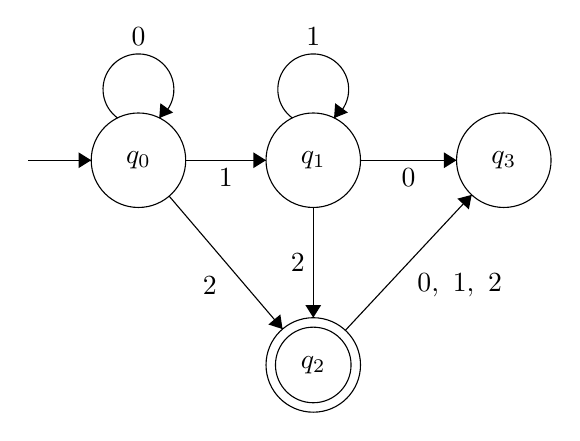
\begin{tikzpicture}[scale=0.2]
          \tikzstyle{every node}+=[inner sep=0pt]
          \draw [black] (7.2,-9) circle (3);
          \draw (7.2,-9) node {$q_0$};
          \draw [black] (18.3,-9) circle (3);
          \draw (18.3,-9) node {$q_1$};
          \draw [black] (18.3,-22) circle (3);
          \draw (18.3,-22) node {$q_2$};
          \draw [black] (18.3,-22) circle (2.4);
          \draw [black] (30.4,-9) circle (3);
          \draw (30.4,-9) node {$q_3$};
          \draw [black] (0.2,-9) -- (4.2,-9);
          \fill [black] (4.2,-9) -- (3.4,-8.5) -- (3.4,-9.5);
          \draw [black] (16.977,-6.32) arc (234:-54:2.25);
          \draw (18.3,-1.75) node [above] {$1$};
          \fill [black] (19.62,-6.32) -- (20.5,-5.97) -- (19.69,-5.38);
          \draw [black] (5.877,-6.32) arc (234:-54:2.25);
          \draw (7.2,-1.75) node [above] {$0$};
          \fill [black] (8.52,-6.32) -- (9.4,-5.97) -- (8.59,-5.38);
          \draw [black] (18.3,-12) -- (18.3,-19);
          \fill [black] (18.3,-19) -- (18.8,-18.2) -- (17.8,-18.2);
          \draw (17.8,-15.5) node [left] {$2$};
          \draw [black] (10.2,-9) -- (15.3,-9);
          \fill [black] (15.3,-9) -- (14.5,-8.5) -- (14.5,-9.5);
          \draw (12.75,-9.5) node [below] {$1$};
          \draw [black] (9.15,-11.28) -- (16.35,-19.72);
          \fill [black] (16.35,-19.72) -- (16.21,-18.79) -- (15.45,-19.43);
          \draw (12.2,-16.94) node [left] {$2$};
          \draw [black] (20.34,-19.8) -- (28.36,-11.2);
          \fill [black] (28.36,-11.2) -- (27.45,-11.44) -- (28.18,-12.12);
          \draw (24.88,-16.96) node [right] {$0,\mbox{ }1,\mbox{ }2$};
          \draw [black] (21.3,-9) -- (27.4,-9);
          \fill [black] (27.4,-9) -- (26.6,-8.5) -- (26.6,-9.5);
          \draw (24.35,-9.5) node [below] {$0$};
        \end{tikzpicture}
      \end{center}

      Then by the closure of regular languages under intersection, we know that $ L \cap L_1 $ will also be regular. Then $ L \cap L_1 = L_2 = \{ 0^n1^n2 \mid n \geq 0 \} $(we take 0 and 1 both to the power of $n$, since $ i = j $, therefore, we have equal number of 0s and 1s). Suppose that $L_2$ is also regular, then the pumping lemma should hold. Consider a string $ s = 0^p1^p2 $. Since $ s \in L_2 $, and $ |s| \geq p $, the pumping lemma guarantees that $s$ can be split into three pieces; $ s = xyz $ such that:\vspace*{-2mm}
      \begin{enumerate}
        \item for each $ i \geq 0 $, $ xy^iz \in L_2 $. \vspace*{-1mm}
        \item $ |y| > 0 $ \vspace*{-1mm}
        \item $ |xy| \leq p $
      \end{enumerate}
      Condition 3 of the pumping lemma guarantees that $y$ can only consist of 0s; \vspace*{-2mm}
      \begin{itemize}
        \item[-] $y$ cannot be a 1, as that would imply $x = 0^p$, then $|xy| > p$, furthermore, then the first part of the string would  more 1's than the second part, which is a contradiction \vspace*{-1mm}
        \item[-] By the same argument as above, $y$ cannot be a combination of a 1's followed by a 2 either as that would imply $x = 0^p$, then $|xy| > p$
      \end{itemize}
      Then $ xy = 0^p $, $ y = 0^m $, and $ x = 0^{p - m} $. Pumping $y$ into the string:
      $$ xyyz = 0^p0^m1^p2 $$ $$ xy^2z = 0^{p + m}1^p2 $$

      This shows that there will inevitably be more 0s than 1s since $ p + m > p $, then $ xy^2z \notin L_2 $. Hence we arrive at a contradiction as the pumping lemme does not hold.

      Then $ L_2 $ is not regular. We know that $L_1$ is regular, therefore, by (2), $L$ is not regular. Hence proved. \vspace*{-2mm}
      \begin{flushright}
        $\blacksquare$
      \end{flushright}
    \end{parts}



  \end{solution}



\end{questions}

\end{document}

%%% Local Variables:
%%% mode: latex
%%% TeX-master: t
%%% End:
